%\documentclass[aastex,a4paper,12pt]{book}
\documentclass[a4paper,11pt]{report}
\usepackage[T1]{fontenc}
\usepackage[utf8]{inputenc}
\usepackage{lmodern}
\usepackage[spanish]{babel}
\usepackage[dvips]{graphics,color,epsfig}
%\usepackage[latin1]{inputenc}

\usepackage{pst-all}
\usepackage{pstricks}

\usepackage{amssymb} % Math
\usepackage{graphicx}
\usepackage{float}
\usepackage{amsmath}
%

% Defino clases de secciones en ESPAÑOL
\def\chaptername{Cap\'\i tulo}
\def\abstractname{Resumen}
\def\contentsname{Contenidos}
\def\bibname{Bibliograf\'\i a}
\def\appendixname{Ap\'endice}
\def\tablename{\textbf{Tabla}}
\def\figurename{\textbf{Figura}}
\usepackage[dvips]{graphics,color,epsfig}
\usepackage{pst-all}
\usepackage{pstricks}
%\usepackage[spanish]{babel}
\usepackage[spanish,es-nodecimaldot]{babel}
\topmargin=-2cm  

\addto\captionsspanish{\def\tablename{Tabla}}


%Paquetes a utilizar
\input{epsf.sty}

\usepackage{amssymb}
%\usepackage[spanish]{babel}
\usepackage[utf8]{inputenc}

\usepackage{amssymb} % Math
\usepackage{graphicx}
\usepackage{float}
%\usepackage{wrapfig}
%\usepackage{deluxetable}

\pagenumbering{arabic}
\usepackage[dvips]{graphics,color}
\usepackage{amssymb} % Math
\usepackage{amsmath} % Math
%\usepackage{dsfont} % Math
\usepackage{float}
\usepackage{graphicx}
\usepackage{wrapfig}
\usepackage{pst-all}
\usepackage{multirow} % Multi filas
\usepackage{multicol}

\usepackage{anysize}
\marginsize{3cm}{3cm}{3cm}{3cm}
\linespread{1.3}

\usepackage{natbib}

%Separacion silabica:
%\usepackage[T1]{babel} % silabas y hyphenation
%\hyphenation{e-vi-den-cia}
%\hyphenation{an-te-rio-res}

% Control de Márgenes

% NAHUEL's
\setlength{\oddsidemargin}{0.5cm}
\setlength{\evensidemargin}{1.5cm}
\setlength{\topmargin}{2cm}
%\setlength{\headheight}{1cm}
%\setlength{\headsep}{1cm}
%\setlength{\topskip}{1.5cm}
\setlength{\textheight}{20cm}
\setlength{\textwidth}{16cm}
%\setlength{\parindent}{1em} % sangria

% ALBERT's
\usepackage{anysize}
\marginsize{2.cm}{2.cm}{0.5cm}{0.75cm} %{left}{right}{top}{bottom}
\marginsize{3.cm}{2.cm}{2cm}{3cm} %{left}{right}{top}{bottom}

\newcommand{\HRule}{\rule{\linewidth}{0.5mm}}

%Font Arial
%\renewcommand{\rmdefault}{phv} % Arial
%\renewcommand{\sfdefault}{phv} % Arial

% Math:
\def\deg{$^\circ$}
\def\rsun{R$_{\odot}$}
\def\bB{\mathbf{B}}
\def\bE{\mathbf{E}}
\def\dpar#1#2{\frac{\partial#1}{\partial#2}}
%color:
\def\red#1{{\textcolor{red}{#1}}}
\def\azul#1{{\textcolor{blue}{#1}}}

\def\fig#1{Figura \ref{#1}}
\def\figa#1#2{Figuras \ref{#1} a \ref{#2}}
\def\figsy#1#2{Figuras \ref{#1} y \ref{#2}}
\def\tabla#1{Tabla \ref{#1}}
\def\eq#1{Ecuaci\'on (\ref{#1})}
\def\eqa#1#2{Ecuaciones (\ref{#1})-(\ref{#2})}
\def\eqn#1{Ecuaci\'on (\ref{#1})}
\def\eqsy#1#2{Ecuaciones (\ref{#1}) y (\ref{#2})}
\def\seccion#1{Sección \ref{#1}}
\def\cap#1{Capítulo \ref{#1}}

\def\exp{{\rm exp}}
\def\ln{{\rm ln}}
\def\sin{{\rm sen}}
\def\cos{{\rm cos}}
\def\sec{{\rm sec}}
\def\erg{{\rm erg}}
\def\cm{{\rm cm}}
\def\km{{\rm km}}
\def\sr{{\rm sr}}
\def\Hz{{\rm Hz}}
\def\GHz{{\rm GHz}}
\def\kev{{\rm kev}}
\def\sfu{{\rm SFU}}
\def\K{{\rm K}}
\def\MK{{\rm MK}}
\def\AU{{\rm UA}}
\def\UA{{\rm UA}}
\def\Log10{{\rm log_{10}}}
\def\G{{\rm G}}
\def\gsun{g_{\odot}}
\def\Rsun{R_{\odot}}
\def\Msun{ M_{\odot}}
\def\Ne{N_\mathrm{e}}
\def\NH{N_\mathrm{H}}
\def\NHe{N_\mathrm{He}}
\def\me{m_\mathrm{e}}
\def\mH{m_\mathrm{H}}
\def\mHe{m_\mathrm{He}}
\def\Tm{T_m}
\def\Tfit{T_{\rm fit}}
\def\Tefit{T_{e,{\rm fit}}}
\def\Te{T_{\rm e}}
\def\TH{T_{\rm H}}
\def\THe{T_{\rm He}}
\def\l{\lambda_{{\rm N}}}
\def\WT{W_{T}}
\def\aTm{\left<\Tm\right>}
\def\dT{\Delta T}
\def\emisin{\zeta_k^{\rm (syn)}}
\def\emitom{\zeta_k^{\rm(tom)}}

\def\fa{f_{\alpha} ({\bf x},{\bf w},t)}
\def\ffa{f_\alpha}
\def\xt{({\bf x},t)}
\def\vt{({\bf v},t)}
\def\xw{({\bf x},{\bf w})}
\def\xwt{({\bf x},{\bf w},t)}
\def\fa{f_\alpha}
\def\ww{{\bf w}}
\def\xx{{\bf x}}
\def\uu{{\bf u}}
\def\kk{{\bf k}}
\def\V{{\bf V}}
\def\ga{{\bf \Gamma}}

\def\lD{\lambda_D}
\def\ve{v_{Te}}
\def\we{\omega_e}
%\def\me{m_e}

\def\dgdv{ \frac{\partial g}{\partial v} }

\def\dndt{ \frac{\partial n}{\partial t} }
\def\drhodt{ \frac{\partial \rho}{\partial t} }

\def\dfdt{ {{\partial f} \over {\partial t}} }
\def\dfdx{ {{\partial f} \over {\partial \xx}} }
\def\dfdw{ {{\partial f} \over {\partial \ww}} }

\def\ddv{ {{\partial} \over {\partial v}} }
\def\ddt{ {{\partial} \over {\partial t}} }
\def\ddx{ {{\partial} \over {\partial \xx}} }
\def\ddw{ {{\partial} \over {\partial \ww}} }

\def\ep{\epsilon}
\def\al{\alpha}
\def\om{\omega}
\def\EF{{\bf E}}
\def\BF{{\bf B}}
\def\dl{\lambda_D}

\def\wp{\om_{pe}}
\def\P{\buildrel =\over P}

\def\intindef{\int_{0}^{\infty}}
%-----------Albert's-----------------
\def\rmax{$R_{\rm max}$}
\def\Nrad{N_r}
\def\Nlat{N_\theta}
\def\Nlon{N_\phi}
\def\bzeta{\boldsymbol{\zeta}}
\def\bI{{\boldsymbol{I}}}
\def\bW{{\bf W}}
\def\bp{{\boldsymbol{p}}}
\def\bR{{\bf R}}
\def\AFe{A_{\rm Fe}}
\def\br{{\bf r}}
\def\bl{{\boldsymbol{\lambda}}}
\def\Tab#1{Tabla \ref{#1}}
\def\Tmin{T_{\rm min}}
\def\Tmax{T_{\rm max}}
\def\intmm{\int_{\Tmin}^{\Tmax}}

\def\Ne0{N_{\rm e0}}
\def\Tm{T_{\rm m}}

\def\ldem{{\rm LDEM}}
\def\trf{{\rm TRF}}
\def\fbe{{\rm FBE}}

\def\Neb{N_{\rm e0}}
\def\lamN{\lambda_{\rm N}}

\def\ba#1{\textcolor{blue}{\bf\tt #1}}
\def\br#1{\textcolor{red}{\bf\tt #1}}
\def\bg#1{\textcolor{green}{\bf\tt #1}}

\def\sdev{{\rm Sdv}}
\def\med{{\rm Med}}
\def\mean{{\rm Mean}}
\def\MK{{\rm MK}}
\def\rsun{R$_\odot$}
\def\mrsun{{\rm R_\odot}}
\def\avgTe{\left<T_e\right>}

\def\lt{$<$}
\def\gt{$>$}

\def\dT{{\rm d}T}
\def\ds{{\rm d}s}
\def\deltat{$\delta$}
\def\Ne{$N_e$}
\def\Te{$T_e$}
\def\lN{$\lambda_N$}
\def\uNe{$10^8{\rm cm}^{-3}$}
\def\mdeg{^\circ}
\def\acs{{\rm ACS}}
\def\acn{{\rm ACN}}
\def\mAA{{\rm \AA}}
\def\mNe{N_e}
\def\mTe{T_e}
\def\mrsunsq{{\rm R^2_\odot}}
\def\corr#1{{\bf #1}}
\def\rojo#1{\textcolor{red}{#1}}



\usepackage{comment}
\usepackage{physics}
\usepackage{url}
\usepackage{natbib}
\def\red#1{{\textcolor{red}{#1}}}
\def\deg{$^\circ$}
\def\rsun{R$_{\odot}$}
\def\fig#1{Figura \ref{#1}}
\def\mrsun{{\rm R_\odot}}
\def\kp{k$_{\rm p}$}
\def\ap{A$_{\rm p}$}
\def\bz{B$_{\rm z}$}
\def\hpt{HP$_{\rm t}$}
\def\hpe{HP$_{\rm e}$}
\def\hpi{HP$_{\rm i}$}
\def\ppe{P$_{\rm e}$}
\def\ppi{P$_{\rm i}$}
\def\vsw{V$_{\rm sw}$}
\def\dsw{D$_{\rm sw}$}
\def\psw{P$_{\rm sw}$}
\def\bt{B$_{\rm t}$}
\def\vbt{VB$_{\rm t}$}
\def\ekl{E$_{\rm kl}$}
\def\rt{${\rm R_T}$}
\def\bvec{$\boldsymbol{B}$}

% Definitions for the journal names
\newcommand{\adv}{    {\it Adv. Space Res.}} 
\newcommand{\annG}{   {\it Ann. Geophys.}} 
\newcommand{\aap}{    {\it Astron. Astrophys.}}
\newcommand{\aaps}{   {\it Astron. Astrophys. Suppl.}}
\newcommand{\aapr}{   {\it Astron. Astrophys. Rev.}}
\newcommand{\ag}{     {\it Ann. Geophys.}}
\newcommand{\aj}{     {\it Astron. J.}} 
\newcommand{\apj}{    {\it Astrophys. J.}}
\newcommand{\apjs}{   {\it Astrophys. J. Suppl.}}
\newcommand{\apjl}{   {\it Astrophys. J. Lett.}}
\newcommand{\apss}{   {\it Astrophys. Space Sci.}} 
\newcommand{\cjaa}{   {\it Chin. J. Astron. Astrophys.}} 
\newcommand{\gafd}{   {\it Geophys. Astrophys. Fluid Dyn.}}
\newcommand{\grl}{    {\it Geophys. Res. Lett.}}
\newcommand{\ijga}{   {\it Int. J. Geomagn. Aeron.}}
\newcommand{\jastp}{  {\it J. Atmos. Solar-Terr. Phys.}} 
\newcommand{\jgr}{    {\it J. Geophys. Res.}}
\newcommand{\mnras}{  {\it Mon. Not. Roy. Astron. Soc.}}
\newcommand{\nat}{    {\it Nature}}
\newcommand{\pasp}{   {\it Pub. Astron. Soc. Pac.}}
\newcommand{\pasj}{   {\it Pub. Astron. Soc. Japan}}
\newcommand{\pre}{    {\it Phys. Rev. E}}
\newcommand{\solphys}{{\it Solar Phys.}}
\newcommand{\sovast}{ {\it Soviet  Astron.}} 
\newcommand{\ssr}{    {\it Space Sci. Rev.}} 
\newcommand{\procspie}{{\it Proc. SPIE}}
\newcommand{\prl}     {{\it Physical Review Letters}}





\title{Monografía Temas Avanzados de Fluidos}
\author{Diego Lloveras}

\begin{document}
\begin{center}

\includegraphics[width=0.3\textwidth]{figuras/Logo-fcenuba.pdf}\\[1cm]
\textsc{\LARGE Universidad de Buenos Aires}\\[0.5cm]
\textsc{\large Facultad de Ciencias Exactas y Naturales}\\[1cm]
%\textsc{  Monografía Dinámica de la alta atmósfera}\\[0.5cm]
%\HRule \\[0.2cm]
\textsc{\LARGE Modelado de ondas del Alfvén turbulentas en el viento solar}\\[1cm]
\textsc{\large DIEGO LLOVERAS}\\[0.7cm]

\textsc{\large Monografía Temas Avanzados de Fluidos}\\[0.5cm]
%\HRule \\[0.1cm]
%\maketitle
\end{center}
%\maketitle
\tableofcontents

\begin{abstract}
El objetivo de esta monografía es introducir los conceptos físicos mínimos necesarios para modelar ondas de Alfvén en el viento solar y la disipación de las mismas en el marco del modelo MHD Alfvén Wave Solar Model (AWSoM). Veremos una breve introducción de las propiedades del viento solar en la Sección \ref{cap1} junto con una propuesta de calentamiento y aceleración del viento solar dado por las ondas de Alfvén. En la Sección \ref{mhd} introduciremos las ecuaciones MHD, las ecuaciones que describen las ondas de Alfvén y veremos los conceptos fenomenológicos mas importantes de la disipación por cascada turbulenta. Finalmente en la Sección \ref{propagacion} veremos como se puede incluir esta disipación en un modelo MHD 3D, donde seguimos en particular lo realizado en AWSoM \citep{vander_2014}.%\textcolor{red}{se muestran resultados del modelo donde queda en evidencia que la idea es buena.}
\end{abstract}

\chapter{Introducción}\label{cap1}
En este capítulo introduciremos algunos conceptos básicos de la corona solar, del viento solar y propondremos a las ondas de Alfvén como mecanismo de calentamiento.
\section{Corona Solar}
La corona solar es la atmósfera exterior del Sol, con una temperatura de 1 a 2 MK es mucho mas caliente que la fotosfera ($\sim 6000K$). Dado que la densidad de la corona ($10^{8} cm^{-3}$) es mucho menor que la de la fotosfera ($10^{17} cm^{-3}$), la densidad de energía térmica de la corona (aunque es 200–300 veces más caliente que la fotosfera) es insignificante en comparación con la densidad de energía fotosférica. 
Dado que no hay una fuente de energía plausible más lejos en la corona para calentar la misma, debemos asumir que existe algún mecanismo (lo mas probable es que sean varios coexistiendo) que transforme energía magnética en calor. Este es el problema del calentamiento coronal, aún sin resolver.


\begin{comment}
\section{Sol}
El Sol es una esfera de  plasma autogravitante. Durante la formación estelar, la presión y la temperatura interna aumentaron generando eventualmente un entorno propicio para el inicio de reacciones nucleares. Estas reacciones, principalmente de fusión de hidrógeno en helio, ocurren en el núcleo del Sol ($T \approx 15$ MK) y son las responsables de la producción de energía. La energía producida viaja en forma de radiación hacia el exterior a través de una zona denominada \emph{zona radiativa} que rodea al núcleo. Luego, debido a variaciones de temperatura y densidad, el plasma solar se torna ópticamente grueso y el transporte neto de energía más eficiente es el convectivo; de tal forma que no hay flujo neto de materia, pero si de energía. A esta zona se la denomina \emph{zona convectiva}. A medida que nos alejamos del centro del Sol, pasando la zona convectiva, la densidad y la temperatura disminuyen y eventualmente el Sol se torna nuevamente ópticamente delgado y por lo tanto el transporte radiativo vuelve a ser eficiente. A esta zona con temperatura del orden de 6000 K se la denomina \emph{fotosfera}. Un esquema del interior solar ese muestra en la Fig \ref{estructura_solar}.

\begin{figure}[ht]
\begin{center}
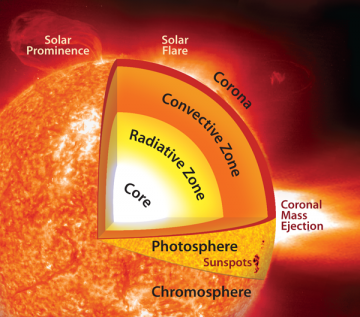
\includegraphics[width=0.65\textwidth]{figuras/SolarStructure.png}
\end{center}
\caption{Estructura interna del sol. Fuente: http://www.nasa.gov/.}
\label{estructura_solar}
\end{figure}


La corona solar es la atmósfera exterior del Sol, con una temperatura de 1 a 2 MK. Aunque la existencia de la corona se conoce desde hace mucho tiempo por los eclipses solares totales, su temperatura de un millón de grados no se reconoció hasta que sus espectros fueron interpretados correctamente por la física de los procesos de radiación en la década de 1940. Entonces se planteó la pregunta de por qué se produce una temperatura tan alta de la corona. Dado que la densidad de la corona ($10^{8} cm^{-3}$) es mucho menor que la de la fotosfera ($10^{17} cm^{-3}$), la densidad de energía térmica de la corona (aunque es 200–300 veces más caliente que la fotosfera) es insignificante en comparación con la densidad de energía fotosférica. 
Dado que no hay una fuente de energía plausible más lejos en la corona para calentar la misma, debemos asumir que existe algún mecanismo (lo mas probable es que sean varios coexistiendo) que transforme energía magnética en calor. Este es el problema del calentamiento coronal, aún sin resolver.

\begin{figure}[ht]
\begin{center}
%\includegraphics[width=0.99\textwidth]{figuras/solar_interior_nasa.jpg}
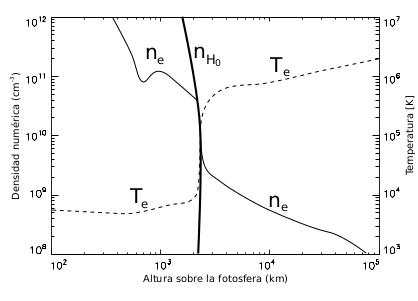
\includegraphics[width=0.65\textwidth]{figuras/calentamiento.png}
\end{center}
\caption{Esquema de la variación de densidad y temperatura con la altura de la atmósfera solar. La línea sólida denota la variación de la densidad de electrones, mientras que la línea a trazos indica la temperatura electrónica.}
\label{calentamiento}
\end{figure}



La Figura \ref{calentamiento} muestra las estructuras de temperatura y densidad de la atmósfera solar. Un límite delgado entre la cromosfera y la corona es llama región de transición, donde la temperatura salta repentinamente de $10^4$ K a $10^6 K$. La región de transición emite radiaciones ultravioleta (UV) y ultravioleta extrema (EUV). La emisión de la corona de 1–2 MK está en el EUV a rangos de rayos X suaves.
La última región es la corona que se extiende desde la región de transición hasta el medio interplanetario y se caracteriza por temperaturas del orden del MK y densidades del orden de $10^8\ - 10^9\ \rm {cm^{-3}}$. Varios fenómenos de interés astrofísico ocurren en distintas regiones de la corona como ser las eyecciones de masa coronal (CMEs por sus siglas en inglés) y las fulguraciones (\fig{estructura_solar}), etc.
\end{comment}

\section{Viento solar}
Los movimientos convectivos debajo de la fotosfera solar generan campo magnético cuyas líneas atraviesan la corona. Gracias a la alta temperatura de la corona, los elementos que la componen se encuentran altamente ionizados y en consecuencia interactúan con el campo magnético del Sol. Como la divergencia del campo magnético es nula, las líneas de campo son cerradas, pero hay distintos tipos. Las más cortas se cierran cerca de la fotosfera y las más largas en el medio interplanetario, a estas últimas las llamaremos abiertas. Los arcos magnéticos influyen fuertemente en el plasma coronal, dejando materia ``atrapada'' en las líneas cerradas y eyectando materia al medio interplanetario siguiendo las líneas abiertas en lo que se llama {viento solar} . El viento solar invade el medio interplanetario, y junto con otros fenómenos como CMEs, tienen un impacto en la magnetósfera terrestre. El modelado y la predicción del clima espacial depende en buena parte de entender los fenómenos físicos que generan el viento solar.

El viento solar es plasma proveniente del sol, es el responsable de mantener la heliósfera y es el agente externo que moldea las magnetosferas planetarias. El viento solar se conforma de una componente altamente variable llamada viento solar lento con velocidades terminales de $\sim 450\pm 100$ km/s y densidades $\sim 10 \rm{ cm^{-3}}$ y se la asocia a regiones de campo magnético cerrado, y de una componente uniforme llamada viento solar rápido con velocidades $\sim 800\pm 100$ km/s y densidades $\sim 3 \rm{ cm^{-3}}$ y se la asocia a regiones de campo magnético abierto.

\begin{figure}[h]
\begin{center}
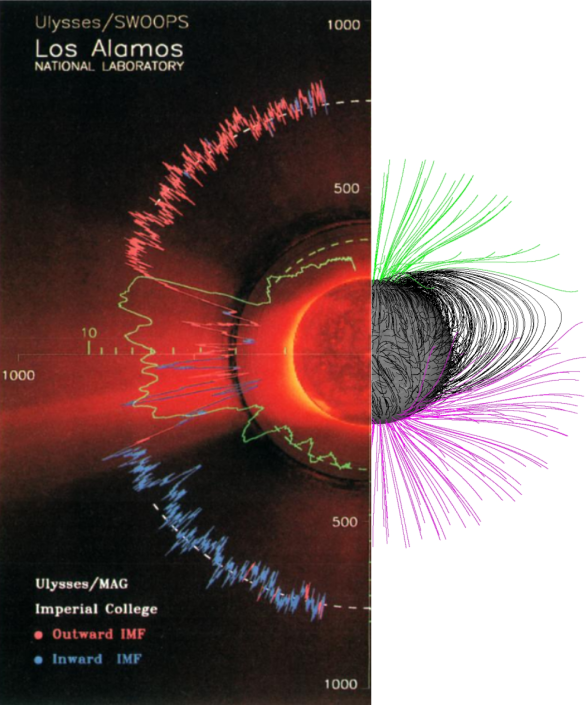
\includegraphics[width=0.7\textwidth]{figuras/mezcla_pfss_ulysses.png}
\end{center}
\caption{Izquierda: La velocidad del viento solar (en rojo y azul) y la densidad en verde, datos tomados con Ulysses. Derecha: líneas de campo magnético realizadas con un modelo potencial con superficie fuente. En negro las líneas magnéticamente cerradas y en verde y magenta las líneas abiertas con distinta polaridad.}
\label{ulysses}
\end{figure}

La Figura \ref{ulysses} muestra dos figuras en una. En la parte izquierda una porción de una figura del paper \citet{mccomas_2000} donde se muestran mediciones in situ de la órbita de Ulysses alrededor del Sol que salió de le eclíptica y paso por la zona polar. Se graficó en rojo y azul la velocidad del viento (cada color indica campo entrante o saliente), y en verde la densidad del viento. La figura de la derecha (creación propia) representa líneas de campo generadas con un modelo potencial con superficie fuente, donde se utilizó como dato un magnetograma (componente radial del campo magnético a nivel fotosférico) durante una época de mínimo de actividad solar. La figura muestra un campo magnético fuertemente dipolar (característico de un mínimo de actividad solar), las líneas negras son las denominadas líneas cerradas (también llamadas Streamer) y las líneas verde y magenta son líneas abiertas (con distinta polaridad). El plasma fluye por las líneas abiertas donde es acelerado y alcanza velocidades terminales altas y densidades bajas, en cambio en las líneas cerradas el campo queda atrapado mayormente y el plasma que escapa conforma el viento solar lento con menor velocidad y mayor intensidad. %El objetivo de este trabajo es introducir los conceptos mas importantes para modelar la corona y el viento solar a gran escala.


\section{Propuesta para calentamiento y aceleración del plasma coronal}

El mecanismo por el cual se calienta la corona solar es un problema fundamental en la astrofísica y la física del plasma, y uno que sigue sin estar completamente explicado. Un mecanismo aceptable transporta energía a la corona, calentándola a temperaturas muy por encima de los valores cromosféricos. Este mecanismo acelera el viento solar y establece las condiciones límite para toda la heliósfera de plasma. %Existen varias limitaciones en un modelo de calentamiento coronal aceptable. (se refiere a observaciones)

Algunos modelos de viento solar apoyan la conclusión de que la aceleración del viento a bajas altitudes requiere un calentamiento bajo en la corona. En los modelos de fluidos, se asume una función de calentamiento ad-hoc Q, que representa la deposición de energía por unidad de volumen como $Q\equiv Q_0 exp[-(r-R_s)/L]$ donde r es la distancia heliocéntrica, $R_s$ es el radio solar, L es la longitud de escala de la disipación y $Q_O \sim 5\times 10^5 ergs ~cm^{-2}s^-1$. A pesar de que no hay evidencia de observación directa de la función de calor exponencial, se sabe que proporciona una rápida aceleración del viento y, con $L \sim 0.3$, explica muchas características observadas de la corona. Aunque se proponen algunas posibles fuentes de calentamiento, en esos modelos no existe un mecanismo físico para explicar esta función de calentamiento y, al ser una cantidad ad-hoc, la expresión exacta de la función exponencial explícita es quizás irrelevante. El punto principal a destacar es el requisito de fuerte calentamiento en el primeros 2 radios solares de la corona. 

\citet{hollweg_1986} propusieron que las ondas se propagan desde la cromosfera hacia el exterior del Sol a bajas frecuencias (como se esquematiza en la Figura \ref{CH}), donde mediante cascadas de tipo turbulento transfieren la energía hacia frecuencias más altas (longitudes de onda mas chica) donde se involucran tasas fenomenológicas turbulentas (del tipo Kolmogorov y Kraichnan) que permiten la disipación y por lo tanto la transferencia de energía.

\citet{dmitruk_2002} demostraron que una distribución de calor puede emerger naturalmente de una cascada turbulenta MHD impulsada por perturbaciones de ondas de Alfvén que se propagan en direcciones opuestas (esto se da naturalmente en la corona baja). Este resultado puede acercarnos a comprender el rompecabezas del calentamiento coronal y el origen del viento solar. Veremos en la Sección \ref{tasa} como puede implementarse esta disipación en un modelo MHD.


%\textcolor{red}{PONER REFERENCIA SECCION} como se implementa la disipación de ondas de Alfvén fuera de la aproximacion WKB dada por \citet{dmitruk_2002}.



\begin{figure}[h]
\begin{center}
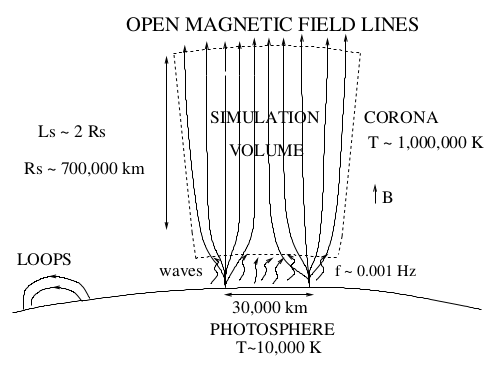
\includegraphics[width=0.7\textwidth]{figuras/dmitruk.png}
\end{center}
\caption{Esquema de ondas propagandose desde la fotosfera hacia la corona a lo largo de líneas abiertas.}
\label{CH}
\end{figure}



\chapter{Magnetohydrodinámica}\label{mhd}

La dinámica de los plasmas confinados magnéticamente, tal como se observa en los sistemas astrofísicos, es esencialmente de naturaleza macroscópica, por lo que se puede estudiar en el modo fluido, veremos a continuación este enfoque. 


La teoría cinética involucra detalles de las funciones de distribución que evolucionan en escalas de tiempo y duración muy cortas, como la longitud de Debye y la frecuencia de plasma. En este trabajo estamos interesados en la dinámica macroscópica de los plasmas magnetizados y bajo ciertas aproximaciones se puede obtener una descripción macroscópica utilizando promedios estadísticos. {Debemos considerar que la escala de tiempo en la que la descripción macroscópica es válida debe ser mayor que el tiempo que tarda en termalizar cada especie.}
%Para eso debemos considerar que la tasa de intercambio de energía entre dos partículas de la misma especie es mucho mayor que entre dos especies diferentes, la tasa de colisión entonces es considerada $\tau_{ii} \gg \tau_{ee} \gg \tau_{ei}$ (el subíndice  indica electrones y el subíndice i indica iones). 
El siguiente paso hacia la descripción macroscópica de un plasma es considerar escalas espaciales grandes (mucho mayor que el radio de ciclotron) y escalas temporales grandes (mucho mayor que la inversa de la frecuencia de ciclotron). Por último la dinámica del plasma debe ser mucho mayor que el tiempo de disipación del campo magnético (esto suele cumplirse incluso en escalas chicas). Con estas consideraciones es posible describir el fluido con un sistema de ecuaciones de dos fluidos, para combinarlos se define la densidad total de masa, la velocidad del centro de masa, la densidad de corriente, la presión y la densidad de carga como:

\begin{eqnarray}
  \rho &\equiv&  n_e m_e + n_i m_i \label{mhd_rho}\\
  \boldsymbol{v} &\equiv& (n_e m_e \boldsymbol{v}_e + n_i m_i \boldsymbol{v}_i) \label{mhd_v} \\
  \boldsymbol{j} &\equiv& -e(n_e \boldsymbol{v}_e + Z n_i \boldsymbol{v}_i) \\
  p &\equiv& p_e + p_i \label{mhd_p}\\
  \tau &\equiv& -e(n_e - Zn_i). \\
\end{eqnarray}
{Como última aproximación al enfoque MHD asumiremos cuasi neutralidad de carga $|n_e - Zn_i| \ll n_e$ y velocidades no relativistas $v \ll c$.}


La descripción física de un sistema hidrodinámico se realiza mediante las leyes de conservación para la masa (o densidad de masa, $\rho$), la densidad de momento ($\rho v$) y la presión del fluido (p). Este conjunto de leyes son las ecuaciones de Euler para fluidos no viscosos, o las de Navier–Stokes para un fluido viscoso. En el caso de un fluido conductor con viscocidad, las ecuaciones de Navier-Stokes se acoplan con las ecuaciones de Maxwell, las cuales describen la evolución del campo electromagnético. Este enfoque nos permite tratar al plasma como un fluido simple conductor y se lo denomina Magnetohidrodinámica (MHD). En la aproximación MHD el plasma es tratado como un gas magnetizado conductor de corriente y eléctricamente neutro. Muchos de los aspectos físicos que caracterizan al plasma se pierden, sin embargo, la descripción es una buena aproximación para muchos problemas en los que los procesos son lentos, es decir en los que las frecuencias son mucho menores que la frecuencia de plasma y es el enfoque más utilizado para describir un plasma en la corona solar. %La teoría de un fluido (MHD) describe un plasma en términos de promedios macroscópicos, es decir, como funciones de posición y tiempo. Para que esta aproximación sea válida, el tamaño, la duración, la densidad y la intensidad del campo magnético deben ser tales que el comportamiento de fluido pueda representarse promediando los fenómenos microscópicos. La escala de tiempo debe ser mayor que el inverso de la frecuencia ciclotrónica, y la escala espacial debe ser mayor que el radio ciclotrónico. Además no se toman en cuenta los efectos de separación de cargas y la diferencia entre las temperaturas de electrones e iones.



\section{Ecuaciones MHD}\label{mhd_ideal}

Las ecuaciones de MHD describen el movimiento de un fluido conductor que interactúa con un campo magnético. Por lo tanto, necesitamos combinar las ecuaciones de Maxwell con las ecuaciones de la dinámica de los gases y proporcionar ecuaciones que describan la interacción.

Primero consideremos las ecuaciones de Maxwell, que describen la evolución del campo eléctrico $\boldsymbol{E}(\boldsymbol{r},t)$ y el campo magnético $\boldsymbol{B}(\boldsymbol{r},t)$ en respuesta a la densidad de corriente $\boldsymbol{j}(\boldsymbol{r},t)$ y a la carga $\tau(\boldsymbol{r},t)$.
\begin{eqnarray}
\nabla \times \boldsymbol{E} &=& -\frac{\partial\boldsymbol{B}}{\partial t} \label{faraday}\\ 
\nabla \cdot \boldsymbol{B} &=& 0 \\
\nabla \times \boldsymbol{B} &=& \mu_0 \boldsymbol{J} + \frac{1}{c^2}\frac{\partial\boldsymbol{E}}{\partial t}\label{ampere}\\
\nabla \cdot \boldsymbol{E} &=& \frac{\tau}{\epsilon_0}. \label{poisson}\\
\end{eqnarray}

Ahora consideremos la ecuación de la dinámica del gas para la evolución de la densidad $\boldsymbol{\rho}(\boldsymbol{r},t)$ y la presión $\boldsymbol{p}(\boldsymbol{r},t)$.
\begin{eqnarray}
\frac{d\rho}{dt} + \rho \nabla \cdot \boldsymbol{v} &\equiv& \frac{\partial \rho}{\partial t} +\nabla \cdot (\rho \boldsymbol{v}) = 0\\
\frac{d p}{dt} + \gamma p \nabla \cdot \boldsymbol{v} &\equiv& \frac{\partial p}{\partial t} + \boldsymbol{v} \cdot \nabla p + \gamma p \nabla \cdot \boldsymbol{v} = 0\\
\end{eqnarray}
donde utilizamos la definición de derivada convenctiva $\frac{d}{dt}=\frac{\partial}{\partial t} + \boldsymbol{v} \cdot \nabla$. 

Hasta el momento los dos sistemas de ecuaciones descriptos por las variables $\boldsymbol{E}, \boldsymbol{B}$ y por $\rho, p$ están desacopladas. Esta interacción se introduce a través de las ecuaciones que involucran el campo de velocidades $\boldsymbol{v}(\boldsymbol{r},t)$ del fluido. Dicha ecuación es el balance de fuerzas por unidad de volumen o conservación del momento dada por,

\begin{equation}
\rho \frac{d\boldsymbol{v}}{dt} = - \nabla p + \boldsymbol{J} \times \boldsymbol{B} +\rho \boldsymbol{g} +\tau \boldsymbol{E}+\nu\nabla^2\boldsymbol{v} \label{momento}
\end{equation}
que representa la aceleración causada por gravedad, gradiente de presión, contribuciones electromagnéticas y el último término $\nu$ es la viscosidad. Notar que si despreciamos las contribuciones electromagnéticas recuperamos Navier-Stokes, y si además despreciamos el término viscoso obtenemos Euler.
Por último añadimos la ley de Ohm en el sistema de laboratorio,
\begin{equation}
\boldsymbol{E'} = \boldsymbol{E} + \boldsymbol{v} \times \boldsymbol{B} = \eta \boldsymbol{j} \label{campo_E}
\end{equation}
donde el último término $\eta$ representa difusividad. En el caso ideal se desprecia este término y obtenemos que el campo eléctrico $\boldsymbol{E'}$ en un marco comovil debe ser nulo.
En este punto el sistema de Ecuaciones (\ref{faraday})-(\ref{campo_E}) puede considerarse completo. Para el plasma que nos interesa a nosotros en este trabajo es suficiente con hacer algunas aproximaciones a estas ecuaciones. Vamos a considerar velocidades no relativistas $v\ll c$ y en ese caso podemos hacer las siguientes estimaciones al orden de magnitud de los diferentes términos de la ecuación de Ampere (Ec. \ref{ampere}).
\begin{equation}
\frac{1}{c^2} \left| \frac{\partial \boldsymbol{E}}{\partial t} \right| \sim \frac{v^2 B}{c^2 l_0} \ll \left| \nabla \times \boldsymbol{B} \right| \sim \frac{B}{l_0}
%\boldsymbol{E'} = \boldsymbol{E} + \boldsymbol{v} \times \boldsymbol{B} = 0 \label{campo_E}
\end{equation}
donde usamos que $v\sim l_0/t_0$ y que $E\sim v B$ (Ec. \ref{campo_E}). En consecuencia podemos despreciar la corriente de desplazamiento en la ley de Ampere.
Al mismo tiempo, la aproximación no relativista implica una simplificación en la ecuación de momentos (Ec. \ref{momento}), ya que

\begin{equation}
\tau \left| \boldsymbol{E} \right| \sim \frac{v^2}{c^2} \frac{B^2}{\mu_0 l_0} \ll \left| \boldsymbol{J} \times \boldsymbol{B}\right| \sim \frac{B^2}{\mu_0 l_0}
\end{equation}
donde hemos usado la Ec. \ref{ampere} habiendo despreciado la corriente de desplazamiento para el término de la derecha, y las Ecuaciones \ref{campo_E} y \ref{poisson} para el término de la izquierda. En consecuencia podemos despreciar la aceleración electrostática dada por las cargas y de esta forma eliminar la ecuación de Poisson (Ec. \ref{poisson}) de nuestro conjunto de ecuaciones.

Reemplazando la Ec. \ref{campo_E} y la ley de Ampere (Ec. \ref{ampere}) en la ley de Faraday (Ec. \ref{faraday}) obtenemos la ecuación de inducción magnética
\begin{equation}
\frac{\partial \boldsymbol{B}}{\partial t} = \nabla \times (\boldsymbol{v} \times \boldsymbol{B}) + \eta \nabla^2 \boldsymbol{B}. \label{induccion}
\end{equation}



De esta forma obtenemos las ecuaciones que componen MHD:
\begin{eqnarray}
\frac{\partial \rho}{\partial t} +\nabla \cdot (\rho \boldsymbol{v}) = 0 \label{conserv_densidad} \\
%\rho \frac{d\boldsymbol{v}}{dt} = - \nabla p + \boldsymbol{J} \times \boldsymbol{B} +\rho \boldsymbol{g} +\tau \boldsymbol{E} \\
\rho \left( \frac{\partial\boldsymbol{v}}{\partial t} + \boldsymbol{v} \nabla \cdot \boldsymbol{v}\right) +\nabla p - \rho \boldsymbol{g} -\frac{1}{\mu_0}(\nabla \times \boldsymbol{B}) \times \boldsymbol{B} =\nu \nabla^2\boldsymbol{v} \label{mhd_momento} \\
%\frac{\partial(\rho\boldsymbol{v})}{\partial t} + \nabla \cdot \left(\rho \boldsymbol{v} \boldsymbol{v} - \frac{\boldsymbol{B}\boldsymbol{B}}{mu_0} \right) +\nabla (p+\frac{B^2}{2\mu_0})=-gGM_\odot\frac{\boldsymbol{r}}{r^3}\label{mhd_momento} \\
\frac{\partial p}{\partial t} + \boldsymbol{v} \cdot \nabla p + \gamma p \nabla \cdot \boldsymbol{v} = 0 \label{presion}\\
\frac{\partial \boldsymbol{B}}{\partial t} - \nabla \times (\boldsymbol{v} \times \boldsymbol{B}) = \eta \nabla^2 \boldsymbol{B} \label{mhd_B} \\
\nabla \cdot \boldsymbol{B} = 0 
\end{eqnarray}
Estas conforman un conjunto de ocho ecuaciones diferenciales parciales no lineales para las ocho variables $\rho(\boldsymbol{r},t)$, $p(\boldsymbol{r},t)$, $\boldsymbol{v}(\boldsymbol{r},t)$ y $\boldsymbol{B}(\boldsymbol{r},t)$. Notar que hemos añadido la gravedad a la ecuación \ref{mhd_momento}
\begin{comment}
Es de interés también elaborar las ecuaciones de evolución para las otras variables termodinámicas, que podrían reemplazar $\rho$ y $p$. Por ejemplo, la energía interna por unidad de masa $e$ (que es equivalente a la temperatura) y la entropía por unidad de masa $s$. Para este trabajo nos resultará útil la primera, que se define utilizando la ecuación de gases ideales $p = (n_e +n_i)kT$,
\begin{equation}
e \equiv \frac{1}{\gamma -1 } \frac{p}{\rho} \approx C_v T \label{ener}
\end{equation}

Si de la Ec. \ref{ener} reemplazamos $p=e (\gamma -1)\rho$ en la Ec. \ref{presion} y utilizamos la Ec. \ref{conserv_densidad} y multiplicamos la ecuación restante por $1/(\gamma -1)e$ obtenemos la ecuación para la energía interna (que reemplazaría a la Ec. \ref{presion} en el set de ecuaciones que conforman MHD ideal),

\begin{equation}
\frac{de}{dt} + (\gamma -1)e\nabla \cdot \boldsymbol{v} =0 \label{conserv_ener}
\end{equation}
\end{comment}


Se puede estimar la importancia de la resistividad comparando los dos términos de la Ec \ref{mhd_B}, para ello definimos el número de Reynold magnético como:
\begin{equation}
R_m = \frac{\nabla \times (\boldsymbol{v} \times \boldsymbol{B}) }{\eta \nabla^2 \boldsymbol{B}} \approx \frac{vL}{\eta}\label{reynold}
\end{equation}
 donde L es una longitud característica de la variación espacial del campo magnético. Cuando el Reynold magnético $R_m$ es grande domina el término no lineal sobre el término difusivo y puede haber un régimen turbulento. De esto se desprende que el fluido arrastra a las líneas de campo y se dice entonces que el campo magnético está ``congelado'' al fluido. 
 
El parámetro que estima el peso de la no linealidad frente a los términos disipativos en el caso hidrodinámico es el número de Reynold cinético
\begin{equation}
R_e = \frac{ \boldsymbol{v}\cdot \nabla \boldsymbol{v}}{\nu \nabla^2 \boldsymbol{v}} \approx \frac{vL}{\nu}\label{reynold_c}.
\end{equation}

En la corona solar tenemos $R_e \gg 1$ y $R_m \gg 1$, con lo cual se espera una dinámica turbulenta. Para un desarrollo formal de la obtención de las ecuaciones MHD el lector puede referirse a \citet{braginskii_1965}. 

\begin{comment}
\section{Inducción magnética}
En el caso de MHD ideal hemos despreciado el término disipativo. Si bien las ecuaciones de de MHD ideal obtenidas en la Sección \ref{mhd_ideal} permiten una generalización directa para incluir el término disipativo debido a la resistividad del plasma, no nos resultará útil obtener las ecuaciones de MHD resistivo. En cambio introduciremos la ecuación de inducción magnética que nos permitirá mas adelante entender como se transfiere energía de por disipación de ondas de Alfvén.

Si tomamos la ley de Ohm (Ec. \ref{campo_E}) considerando el término resistivo tenemos,
\begin{equation}
\boldsymbol{E'} = \boldsymbol{E} + \boldsymbol{v} \times \boldsymbol{B} = \eta \boldsymbol{j} \label{campo_E_resis}
\end{equation}
donde ahora se tiene en consideración la disipación Ohmica a través de la resistividad $\eta$ del plasma.
Reemplazando la Ec. \ref{campo_E_resis} y la ley de Ampere (Ec. \ref{ampere}) en la ley de Faraday (Ec. \ref{faraday}) obtenemos la ecuación de inducción magnética
\begin{equation}
\frac{\partial \boldsymbol{B}}{\partial t} = \nabla \times (\boldsymbol{v} \times \boldsymbol{B}) + \eta \nabla^2 \boldsymbol{B}. \label{induccion}
\end{equation}
%donde hemos definido la constante de difusión magnética como $\eta = c^2/4\pi \sigma$. 
La evolución del campo magnético y de velocidades viene dado por las ecuaciones \ref{momento} y \ref{induccion}, que se encuentran fuertemente acoplados y tiene términos no lineales.
Se puede estimar la importancia de la resistividad comparando los dos términos, para ello definimos el número de Reynold magnético como:
\begin{equation}
R_m = \frac{\nabla \times (\boldsymbol{v} \times \boldsymbol{B}) }{\eta \nabla^2 \boldsymbol{B}} \approx \frac{vL}{\eta}\label{reynold}
\end{equation}
 donde L es una longitud característica de la variación espacial del campo magnético. Cuando el fluido esta en reposo o bien cuando las velocidades son pequeñas, predomina el segundo término de la derecha en la ecuación de inducción. Esto implica que una configuración inicial del campo magnético disminuirá con un tiempo de difusión $t_d\approx L^2/\eta$. Este tiempo de difusión es mucho mas grande que el observado en estructuras de la corona solar, lo que indica que la disipación es acelerada por otro mecanismo.
 
Por otro lado, cuando la difusividad es baja, es decir $R_m$ grande, la Ec. \ref{induccion} se lee como $\frac{\partial \boldsymbol{B}}{\partial t} = \nabla \times (\boldsymbol{v} \times \boldsymbol{B})$ y expresa la conservación del flujo magnético que atraviesa una curva cerrada que se mueve con la velocidad local del fluido. De esto se desprende que el fluido arrastra a las líneas de campo y se dice entonces que el campo magnético está ``congelado'' al fluido. La noción de las líneas de campo arrastradas por el fluido son solo una imagen pictórica, ya que las líneas de campo son una idealización, que indica la dirección del campo local en un instante. El hecho de que las líneas sean arrastradas corresponde a que se generan corrientes que modifican el campo para que su dirección (instante a instante) cambie. A la congelación del campo a la materia se la conoce como teorema de Alfvén.
\begin{comment}
\textcolor{red}{
Podemos ver que el flujo de  líneas de campo magnético se conserva al integrar la ley de Ohm sobre una curva cerrada e igualandola con la forma integral de la ley de Faraday, obtenemos
\begin{equation}
  \oint_{C} (\boldsymbol{E}+\boldsymbol{v}\times \boldsymbol{B})\, d\boldsymbol{r} =\eta \oint_{C} \boldsymbol{J} \, d\boldsymbol{r} = - \frac{d}{d} \int_S \boldsymbol{B} \, d\boldsymbol{S}
\end{equation}
y en el límite de conductor perfecto (MHD ideal) sin difusión obtenemos
\begin{equation}
\frac{d}{dr} \oint_S \boldsymbol{B} d\boldsymbol{S} = 0 \, ,   \,   \,   \,  \eta \rightarrow 0,
\end{equation}
 y de esta forma el flujo se conserva.
 La derivada convectiva de un elemento de fluido es la siguiente
\begin{equation}
  \frac{d}{dt} d\boldsymbol{r} = \boldsymbol{v}(\boldsymbol{x} + d\boldsymbol{r})-\boldsymbol{v}(\boldsymbol{x})=(d\boldsymbol{r}\cdot \nabla) \boldsymbol{v}, 
\end{equation}
donde $d\boldsymbol{r}$ representa un diferencial de elemento de fluido que se desplaza desde $\boldsymbol{x}$ a $\boldsymbol{x}+d\boldsymbol{r}$.
La misma ecuación define el campo magnético sin difusión,
\begin{equation}
  \frac{d}{dt} \boldsymbol{B} = (\boldsymbol{B}\cdot \nabla) \boldsymbol{v}. 
\end{equation}
De esta forma podemos notar que $\boldsymbol{B}$ y $d\boldsymbol{r}$ estan gobernados por la misma ecuación, y por lo tanto deben evolucionar de la misma manera, es decir que las líneas de campo $\boldsymbol{B}$ evolucionan igual que las líneas materiales.
}
%\textcolor{red}{Por lo tanto, el flujo magnético a través de un elemento de superficie que se mueve conjuntamente es constante. Pero, dado que esto es válido para cualquier elemento de la superficie, se conserva el flujo a través de cualquier superficie limitada por un contorno C que se mueve con el fluido.}

\textcolor{red}{para que pongo esto?}
\end{comment}



\section{Ondas de Alfvén}\label{seccion_alfven}

El calentamiento coronal es hasta hoy en día un tema abierto. La imposibilidad de realizar mediciones in-situ en las proximidades de la fotosfera ralentizan el avance en esta área. Distintos fenómenos físicos que se saben ocurren en la corona coexisten simultáneamente y liberan energía calentando la corona y acelerando el viento solar, por ejemplo reconexión magnética, nanofulguraciones, disipación de ondas de Alfvén, etc. Veremos a continuación esta última y como implementarla en nuestro modelado del viento solar y además como introducirlo en en las ecuaciones MHD que mencionamos anteriormente.


En un plasma existen distintos tipos de ondas, en particular si despreciamos la gravedad en las ecuaciones de MHD ideal (despreciando viscosidad y difusividad), las ondas resultan de perturbaciones del campo presión, densidad, velocidad y campo magnético. Cada tipo de onda tiene asociada su correspondiente relación de dispersión y es producida por una fuerza restitutiva. %Veremos a continuación las onda magnéticas compresionales denominadas ondas de Alfvén.

Cuando una línea de campo magnético se ve deformada debido a fluctuaciones en el campo de velocidades, la curvatura resultante da lugar a tensión de Faraday (fuerza restitutiva, $\sim B^2$) que tiende a enderezar la línea. Dado que para $R_m >> 1$ las líneas están congeladas a la materia, se podría considerar que hay cierta inercia y por lo tanto parece intuitivo esperar ondas transversales en el campo magnético. 




Para ilustrar esta idea consideraremos una perturbación $\delta \rho, \delta \boldsymbol{v},\delta p, \delta \boldsymbol{B}$ pequeñas con respecto a su estado base $\rho,  \boldsymbol{v}, p$ y $\boldsymbol{B}$. Reemplazamos las perturbaciones en las ecuaciones de MHD ideal y linealizando obtenemos:

\begin{eqnarray}
  \frac{\partial}{\partial t} \delta \rho_0 &=& - \rho_0 \nabla \cdot \delta \boldsymbol{v}\\
  \rho_0 \frac{\partial}{\partial t} \delta \boldsymbol{v} &=& -\nabla \delta p + (\nabla \times \delta \boldsymbol{B})\times \boldsymbol{B_0} \label{pertu1}\\
  \frac{\partial}{\partial t} \delta p &=& -\gamma p_0 \nabla \cdot \delta \boldsymbol{v}\\
  \frac{\partial}{\partial t} \delta \boldsymbol{B} &=& \nabla \times (\delta \boldsymbol{v}\times \boldsymbol{B_0}) \label{pertu2}.  
\end{eqnarray}
La primera ecuación que determina $\delta \rho$ esta desacoplada. Considerando que estamos interesados en las perturbaciones magnéticas, podemos elegir $p=0$ y de esta forma queda definido $\delta p=0$. Tomando la derivada temporal de la Ec. \ref{pertu1} y reemplazando en ella la Ec. \ref{pertu2} obtenemos una ecuación de onda para la perturbación en velocidad:
\begin{equation}
  \rho_0 \frac{\partial^2 \delta \boldsymbol{v}}{\partial t^2}=\Bigg(\nabla \times \frac{\partial \delta \boldsymbol{B}}{\partial t} \Bigg) \times \boldsymbol{B_0}= \boldsymbol{B_0} \times \Bigg( \nabla \times \Bigg( \nabla \times (\boldsymbol{B_0}\times \delta \boldsymbol{v}) \Bigg) \Bigg).
\end{equation}
Utilizando como solución una onda plana
\begin{equation}
  \delta \boldsymbol{v}(\boldsymbol{r},t)=V e^{i(\boldsymbol{k}\boldsymbol{r}-wt)}
\end{equation}
se obtienen como solución ondas transversales ($\delta\boldsymbol{v}\perp \boldsymbol{B}_0$) que se propagan en al dirección del campo magnético ($\boldsymbol{k} \parallel \boldsymbol{B}_0$). Estas ondas tienen la relación de dispersión $w=\pm k_{\parallel} v_A$  donde se define la velocidad de Alfvén como  $v_A=\frac{\boldsymbol{B}_0}{\sqrt \mu_0 \rho_0}$. Las ondas de Alfvén son causadas por la tensión de las líneas de campo magnético, las cuales tienden a restaurar la forma inicial.


\subsection{Variables de Elsässer}

Introducimos a continuación las variables de Elsässer \citep{elsasser_1950} con las cuales por un lado podremos desacoplar las ecuaciones de MHD ideal y por otro lado nos permitirán representar de forma sencilla las ondas de Alfvén. Estas variables son:
\begin{equation}
  \boldsymbol{z}^\pm = \boldsymbol{v} \pm \frac{\boldsymbol{B}}{\sqrt{\mu \rho}},
\end{equation}
donde $\boldsymbol{v}$ y $\boldsymbol{B}$ representan el vector velocidad y campo magnético respectivamente.
%, el signo positivo indica propagación en la misma dirección que el campo magnético y el signo negativo en dirección opuesta.
Haciendo uso de estas variables y considerando incompresibilidad ($\nabla \cdot \boldsymbol{v}=0$) es posible reescribir el sistema de ecuaciones de MHD ideal (\ref{conserv_densidad}) - (\ref{mhd_B}) de la siguiente forma:

\begin{eqnarray}
  \frac{\partial \boldsymbol{z}^+}{\partial t}+ \boldsymbol{z}^- \cdot \nabla \boldsymbol{z}^+ &=& -\nabla(p + \boldsymbol{B}^2/2\mu) \label{pertu1} \\
  \frac{\partial \boldsymbol{z}^-}{\partial t}+ \boldsymbol{z}^+ \cdot \nabla \boldsymbol{z}^- &=& -\nabla(p + \boldsymbol{B}^2/2\mu)\\
  \nabla \cdot \boldsymbol{z}^\pm &=& 0. \label{pertu3}
\end{eqnarray}
%Los pasos detallados de la reescritura de las ecuaciones MHD en variables de Elsässer pueden encontrarse en \citet{elsasser_1950}. En este punto la única consideración realizada es incompresibilidad ($\nabla \cdot \boldsymbol{v}=0$).

Proponemos pequeñas perturbaciones ($\delta$) en el campo de velocidad y el campo magnético sobre el equilibrio (dado por $v_0 = 0; B=B_0$), es decir $\boldsymbol{B} = \boldsymbol{B}_0 + \delta \boldsymbol{B}$ y $\boldsymbol{v} = 0 + \delta \boldsymbol{v}$ y reescribimos las variables de Elsässer,

\begin{equation}
  \boldsymbol{z}^\pm = \boldsymbol{z}^\pm _0 + \boldsymbol{\delta z} ^\pm = \pm V_{A0} + \boldsymbol{\delta v} \pm \frac{\boldsymbol{\delta B}}{\sqrt{\mu \rho_0}}
\end{equation}
donde $V_{A0} = \boldsymbol{B}_0/\sqrt{\rho \mu_0}$ es la velocidad de Alfvén y hemos usado la perturbación escrita en variables de Elsässer ($\boldsymbol{\delta z} ^\pm = \boldsymbol{\delta v} \pm \frac{\boldsymbol{\delta B}}{\sqrt{\mu \rho_0}}$). Reemplazando esta nueva variable con perturbaciones en las ecuaciones (\ref{pertu1})-(\ref{pertu3}), despreciando $\partial (\boldsymbol{z_0} ^\pm)/\partial t=0$ y despreciando las variaciones espaciales de $\boldsymbol{z_0}$, obteniendo:
\begin{equation}
  \frac{\partial \boldsymbol{z}^\pm}{\partial t}\mp (V_{A}\cdot \nabla)\boldsymbol{z}^\pm+(\boldsymbol{z}^\mp \cdot \nabla)\boldsymbol{z}^\pm= -\nabla(p + \boldsymbol{B}^2/2\mu), \label{pertu_f} 
\end{equation}
donde ahora $\boldsymbol{z}$ lo usamos para indicar perturbación.

Notar que si consideramos ondas propagantes en una sola dirección estas ecuaciones se desacoplan y obtenemos las ecuaciones que describen ondas de Alfvén propagándose paralela o antiparalelamente al campo magnético  \citep{magyar_2019}. %Para una descripción mas detallada de la naturaleza de las variables de 
Supongamos dos perturbaciones localizadas que se propagan en sentido opuesto con una determinada energía inicial y sin interacción. Cuando se superponen, el término no lineal $(\boldsymbol{z}^\mp \cdot \nabla)\boldsymbol{z}^\pm$ comienza tomar partido y las ondas se distorsionan unas a otras (ver Sección \ref{turbulencia}). La energía total final se conservará, pero la distribución espectral de energía cambiará. Es entonces razonable suponer que luego de múltiples interacciones entre distintas ondas, la energía (en promedio) pasará hacia escalas mas chicas durante la colisión, {es decir números de onda mayores que los que tenía cada onda originalmente}, llegando eventualmente a la disipación. Esta sería la esencia de la disipación de ondas de Alfvén. Veremos en la siguiente sección una explicación fenomenológica para esta distribución espectral de energía durante la interacción entre ondas y finalmente la disipación de las mismas.





\section{Cascada de energía de Richardson y microescalas de Kolmogorov} \label{turbulencia}


En esta sección introduciremos una descripción fenomenológica de la transferencia de energía mediante la cual la turbulencia generada por las ondas de Alfvén disipa energía. No se pretende hacer un desarrollo extenso de este tema, sino mas bien dar una idea mas bien fenomenológica de lo que conforma la base de la teoría de la cascada de energía de Kolmogorov para pequeñas escalas. El desarrollo formal puede encontrarse en \citet{kolmogorov_1941} y una explicación mas amigable en \citet{davidson_2013}.




Utilizaremos los símbolos $\ell$ y $\eta$ para representar los valores característicos de las escalas de longitud más grande y más pequeña en la turbulencia, y los símbolos \emph{u} y $\upsilon$ para representar los valores característicos de las fluctuaciones de velocidad de los remolinos de escala  $\ell$ y $\eta$ respectivamente. Las cantidades  $\ell$ y \emph{u} se conocen como escalas integrales de la turbulencia, mientras que $\eta$ y $\upsilon$ se denominan microescalas. En un flujo típico, las escalas integrales se establecen por la geometría general o un forzado externo (inyección de energía), mientras que $\eta$ y $\upsilon$ están determinadas por procesos dinámicos dentro de la turbulencia.

La ley cero de la turbulencia establece que en el límite de Re$\rightarrow \infty$, la tasa media de disipación de energía cinética $\epsilon$, es finita, independiente de $\upsilon$, y depende solo de las escalas integrales $\ell$ y \emph{u}. El análisis dimensional indica que

\begin{equation}
  \epsilon \sim \emph{u}^3 / \ell.
\end{equation}

Por otro lado la disipación viscosa, $\nu S_{ij}S_{ij}$ (donde utilizamos el tensor $S_{ij}=\frac{1}{2}[\frac{\partial v_i}{\partial x_j}+\frac{\partial v_j}{\partial x_i}]$)\footnote{La viscosidad representada por $\nu$ proviene de la ecuación de Navier-Stokes.} en un flujo turbulento es mas pronunciado en los vórtices mas pequeños, donde los gradientes de velocidad son mayores. De esta forma el análisis dimensional indica que
\begin{equation}
  \epsilon \sim \emph{u}^3 / \ell \sim \nu(\upsilon/\eta)^2,
\end{equation}
la cual vincula las escalas integrales con las microescalas.
Entonces, la energía cinética entra en la turbulencia en las escalas más grandes y sale en las escalas más pequeñas, donde se convierte en calor. Decimos que hay un flujo de energía de los vórtices grandes a los pequeños. Hablamos de un flujo de energía a través del espacio de escala. Seguiremos el concepto fenomenológico de la cascada de energía de Richardson esquematizada en la Figura \ref{kolmogorov}. La energía pasa de vórtices grandes a otros mas pequeños en múltiples pasos. Digamos que de los vórtices de inyección $\ell_i$ pasa a $\ell_0$, luego a $\ell_1$ y así sucesivamente hasta $\ell_n$ ($\ell_i>\ell_0>\ell_1>...>\ell_n=\eta$), donde finalmente la energía cinética es transformada en calor.
Cuando $Re=u\ell/\nu >>1$ las fuerzas viscosas que actúan en vórtices con escalas $\ell$ mucho mas grandes que $\ell_n$ son despreciables y la cascada se da por inercia (domina el término). Este proceso se detiene cuando las fuerzas viscosas son del mismo orden que el término inercial, donde la energía cinética puede ser convertida eficientemente en calor. Esto sucede cuando se alcanza la micro escala $\ell_n$ que debe satisfacer $\upsilon \eta/ \nu \sim 1$. Se puede pensar a la cascada de energía como una serie de inestabilidades sucesivas debidas a los términos no lineales entre las escalas de inyección $\ell_i$ y las disipativas $\eta$, alcanzando finalmente un balance entre la energía que ingresa al sistema y la que se disipa.


\begin{figure}[ht]
\begin{center}
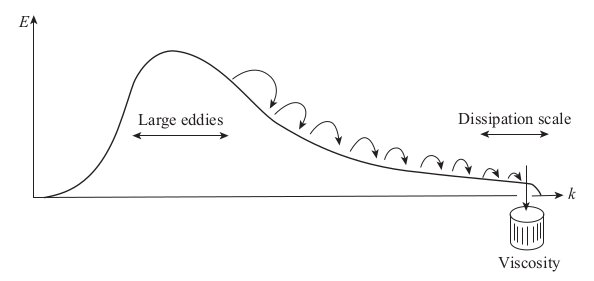
\includegraphics[width=0.85\textwidth]{figuras/kolmogorov2.png}
\end{center}
\caption{Diagrama esquemático de la cascada de energía por multipasos de Richardson \citep{davidson_2013}.}
\label{kolmogorov}
\end{figure}

Para expresar la energía de la perturbación a lo largo de las diferentes escalas debemos utilizar el espacio de Fourier. De esta forma es posible encontrar una expresión para la energía $E(k)$ en función del número de onda $k$. En particular $E(k)$ tiene una contribución finita en el rango $0 <k <\pi/\ell$, que es la suma de todas las colas de baja k de los diferentes espectros correspondientes a los diversos rangos de tamaño. De esta manera, $E(k)$ no es cero en el rango $\pi/\eta<k<\infty$. Dado que no hay remolinos en ninguno de estos dos rangos, no podemos interpretar $E(k)$ como la energía de los remolinos.

La forma típica de $E(k)$ a Re grandes es la siguiente. En el rango $k\ll \pi/\ell$ va como $E(k)\sim k^2$ o bien como $E(k)\sim k^4$ y alcanza el pico en $k\sim \pi/\ell$. Luego en el rango $\pi/\ell \ll k \ll \pi/\eta$ decae como 
\begin{equation}
E(k)\sim \epsilon^{2/3}k^{-5/3} \label{kolmo}
\end{equation}
y finalmente en el rango $k\gg \pi/\eta$ decae exponencialmente.

Las estructuras en la microescala de Kolmogorov evolucionan con un tiempo característico mucho menor que las estructuras de gran escala $\eta/\upsilon \sim (\ell/u)(u\ell/\nu)^{-1/2} \ll \ell/u$, es decir que evolucionan mucho mas rápido en relación a las escalas grandes. A medida que Re aumenta, las escalas divergen $\eta \sim (u\ell/\nu)^{-3/4}\ell \sim Re^{-3/4} \ell$ y consecuentemente la energía contenida en vórtices ocupa diferentes rangos de número de onda. Esto sugiere un desacople entre escalas.

\subsection{Espectro de Kraichnan}
El concepto introducido por Kolmogorov se enfoca en hidrodinámica, y como en esta monografía nos interesa plasma MHD, debemos mencionar el enfoque fenomenológico de Iroshnikov y Kraichnan. El cual considera interacciones entre vórtices turbulentos y ondas de Alfvén que viajan a lo largo del campo magnético medio, a esto se lo suele llamar turbulencia Aflvénica. Introduciremos una teoría fenomenológica del rango inercial que predice la variación por escala en la energía de las fluctuaciones, en otras palabras es una especie de versión MHD del análisis de Kolmogorov (\citet{iroshnikov_1964}; \citet{kraichnan_1965}). Como primera aproximación ignoraremos anisotropía y consideraremos pequeñas turbulencias. Nos enfocaremos en el rango inercial $\eta \ll \lambda \ll \ell$ donde mantenemos la notación anterior, es decir que $\eta$ y $\ell$ representan las escalas de disipación e integrales, respectivamente.

Durante un única interacción entre ondas localizadas, de la Ecuación \ref{pertu_f} se desprende $|\delta \boldsymbol{z}^\pm|\sim |(\boldsymbol{z}^\mp \cdot \nabla \boldsymbol{z}^\pm)|\frac{\lambda_{\parallel}}{V_A}$ donde $\lambda_{\parallel}/V_A$ es el tiempo de interacción donde el numerador es la escala de longitud de las ondas (paralelas al campo). Consideremos una única colisión donde parte de la energía es transferida de la escala $\lambda$ a escalas adyacentes,
\begin{equation}
  |\delta \boldsymbol{z}^\pm|\sim \frac{|\boldsymbol{z}^\mp| |\boldsymbol{z}^\pm|}{\lambda_\perp}\frac{\lambda_{\parallel}}{V_A} \label{yoquese}
\end{equation}
donde $\lambda_\perp$ es la escala transversal al campo. Si despreciamos anisotropía $\lambda_{\parallel}\sim \lambda_{\perp}\sim \lambda$ y consideramos que los paquetes de onda interactuantes satisfacen $|\boldsymbol{z}^+|\sim|\boldsymbol{z}^-|\sim u_\lambda$ y reemplazamos en \ref{yoquese} obtenemos
\begin{equation}
  \delta u_{\lambda} \sim u_{\lambda}^2/\upsilon_{a}.
\end{equation}
Considerando que el tiempo de transferencia de energía característico $\tau_{\lambda}\sim \lambda \upsilon_a/u_{\lambda}^2$ y que el flujo de energía a travez de la cascada es $\pi \sim u_{\lambda}^2/\tau$ y que además es igual a la tasa de disipación $\pi \sim \epsilon$, podemos ver que
\begin{equation}
  u_{\lambda}^2\sim \sqrt{\epsilon \upsilon_a} \lambda^{1/2}.
\end{equation}
Como el espectro de energía va como $kE(k)\sim u_{\lambda}$ y además $\lambda \sim k^{-1}$, entonces obtenemos
\begin{equation}
  E(k)\sim \sqrt{\epsilon}k^{-3/2}. \label{kraichnan}
\end{equation}

En la práctica puede resultar difícil diferenciar entre la potencia de los espectros de Kolmogorov $E(k)\sim k^{-5/3}$ dado por Ec. \ref{kolmo} y los espectros de Kraichnan $E(k)\sim k^{-3/2}$ dado por la Ec. \ref{kraichnan} (\citet{saddoughi_1994}; \citet{bruno_2005}).

Si bien en esta monografía despreciamos la anisotropía en la corona y en el viento solar por simplicidad, esta existe y tiene un impacto en la temperatura protónica \citep{vasquez_2003} que debe ser tenida en cuenta a la hora de realizar un modelo MHD.



\chapter{Propagación, reflexión y disipación de ondas de Alfvén}\label{propagacion}
En esta sección, derivamos las ecuaciones de densidad de energía de las ondas de Alfvén. En la Sección \ref{wkb} derivaremos la ecuación de transporte de ondas (aproximación WKB) en ausencia de reflexión y disipación de ondas. La tasa de disipación no lineal se analiza en la Sección \ref{tasa}, donde además se añade un término para la reflexión de onda.


\section{Ecuación de WKB para las densidades de energía de las ondas turbulentas de Alfvén}\label{wkb}
En esta sección queremos derivar las ecuaciones que gobiernan la evolución de la densidad de energía de onda ($w_{\pm}$). Reescribimos la forma no conservativa de las ecuaciones de momento (Ec. \ref{mhd_momento}) y de campo magnético (Ec. \ref{mhd_B}) que conforman la MHD ideal.

\begin{eqnarray}
  \frac{\partial \boldsymbol{v}}{\partial t} + (\boldsymbol{v} \cdot \nabla) \boldsymbol{v} + \frac{\nabla B^2}{2\mu_0 \rho}+ \frac{\nabla (P_e +P_i)}{\rho} &=& \frac{(\boldsymbol{B} \cdot \nabla)\boldsymbol{B}}{\mu_0 \rho} -\frac{GM_{\odot}}{r^3}\boldsymbol{r} \label{pre1} \\
  \frac{\partial \boldsymbol{B}}{\partial t}+(\boldsymbol{v} \cdot \nabla )\boldsymbol{B} +\boldsymbol{B} (\nabla \cdot \boldsymbol{v}) &=& (\boldsymbol{B} \cdot \nabla)\boldsymbol{v} \label{pre2} 
\end{eqnarray}

Si representamos el campo magnético y la velocidad como suma de parte regular y turbulenta, es decir $\boldsymbol{v}=\tilde{\boldsymbol{v}}+ \delta \boldsymbol{v}$ y $\boldsymbol{B}=\tilde{\boldsymbol{B}}+ \delta \boldsymbol{B}$ (omitiremos los tildes de ahora en mas por simplificación) y simplificamos las ecuaciones al asumir condiciones de incompresibilidad $\nabla \cdot \delta \boldsymbol{v}=0$ y $ \boldsymbol{B}\cdot \delta \boldsymbol{B}=0$  y reescribimos las Ecuaciones \ref{pre1}-\ref{pre2} junto con la conservación de masa, obtenemos


\begin{equation}
\begin{split} 
\frac{\partial \delta \boldsymbol{v}}{\partial t} +(\boldsymbol{v}\cdot \nabla)\delta\boldsymbol{v}  +(\delta \boldsymbol{v} \cdot \nabla)\delta\boldsymbol{v}+&(\delta\boldsymbol{v}\cdot \nabla)\boldsymbol{v}= \\
\frac{(\boldsymbol{B}\cdot \nabla )\delta B}{\mu_0 \rho}+&\frac{(\delta\boldsymbol{B} \cdot \nabla)\delta \boldsymbol{B}}{\mu_0 \rho}+\frac{(\delta\boldsymbol{B}\cdot \nabla)\boldsymbol{B}}{\mu_0 \rho} \label{pertu_v1}
\end{split}
\end{equation}


\begin{equation}
\begin{split} 
\frac{\partial \delta \boldsymbol{B}}{\partial t} +(\boldsymbol{v}\cdot \nabla)\delta\boldsymbol{B}  +(\delta \boldsymbol{v} \cdot \nabla)\delta\boldsymbol{B}+&(\delta\boldsymbol{v}\cdot \nabla)\boldsymbol{B} + \delta \boldsymbol{B}(\nabla \cdot \boldsymbol{v})= \\
(\boldsymbol{B}\cdot \nabla)\delta\boldsymbol{v}  +(\delta \boldsymbol{B} \cdot \nabla)\delta\boldsymbol{v}&+(\delta\boldsymbol{B}\cdot \nabla)\boldsymbol{v} \label{pertu_v2}
\end{split}
\end{equation}

\begin{eqnarray}
  \frac{\partial \rho}{\partial t}+(\boldsymbol{v}\cdot \nabla)\rho+(\delta \boldsymbol{v}\cdot \nabla) \rho + \rho\nabla \cdot \boldsymbol{v} = 0. \label{pertu_v3}
\end{eqnarray}

Las ecuaciones para las variables de Elsässer se obtienen sumando Ec. \ref{pertu_v1} $\pm \frac{1}{\sqrt{\mu_o \rho}}\times$ Ec. \ref{pertu_v2} $\pm \frac{\delta \boldsymbol{B}}{\rho \sqrt{\mu_0 \rho}}\times$ Ec. \ref{pertu_v3}, dando como resultado:

\begin{equation}
  \frac{d_\pm \boldsymbol{z}_\pm}{dt}+ \boldsymbol{z}_\mp \cdot \nabla \boldsymbol{v} \mp \frac{1}{\sqrt{\mu_0 \rho}}(\boldsymbol{z}_\mp \cdot \nabla \boldsymbol{B}) - \frac{1}{4\rho}(\boldsymbol{z}_\pm - \boldsymbol{z}_\mp) \frac{d_\mp \rho}{dt}=0 \label{bardo}
\end{equation}
donde estamos utilizando la derivada total diferenciando ondas propagantes en ambas direcciones $d_\pm/dt = \partial/\partial t+ (\boldsymbol{v}\pm \boldsymbol{V}_A+\boldsymbol{z}_\mp)\cdot \nabla$

Las ondas de Alfvén ejercen presión isotrópica (ver Ec. 21 en \citet{jacques_1977}), la relación entre la presión de onda y la densidad de energía de onda es $P_A = (\delta \boldsymbol{B})^2/2\mu_0$. Despejando $\delta \boldsymbol{B}$ como combinación lineal de $\boldsymbol{z}_+$ y $\boldsymbol{z}_-$ obtenemos:

\begin{equation}
  P_A = \frac{(\delta \boldsymbol{B})^2}{2\mu_0} = \frac{\rho}{4} \Bigg( \frac{\boldsymbol{z}_+^2}{2}+ \frac{\boldsymbol{z}_-^2}{2}+\boldsymbol{z}_+\cdot\boldsymbol{z}_- \Bigg)
\end{equation}

%Esta presión aporta en la aceleración del viento solar y debe ser considerada en la ecuación de momento (Ec. \ref{momento}) junto con los otros términos de presión isótropa. De esta forma, siguiendo los pasos para la obtención de las ecuaciones de conservación mencionado en la Sección \ref{leyes_conserv}, el término $p_A$ aparecerá en las ecuaciones de conservación del momento (Ec. \ref{conserv_momento}) y de la energía (Ec. \ref{energia}), detalladas explícitamente en la Sección \ref{chap_awsom}.

La densidad de energía viene dada por $w_\pm = \rho \boldsymbol{z}_\pm ^2/4$, y las ecuaciones para la densidad de energía se obtienen sumando $\rho \boldsymbol{z}_\pm/2 ~\times$ Ec. \ref{bardo} $+ ~3\boldsymbol{z}_\pm^2/8 ~\times$ Ec. \ref{pertu_v3}:

\begin{equation}
\begin{split} 
\frac{\partial w_\pm}{\partial t} + \nabla \cdot [(\boldsymbol{v} \pm \boldsymbol{V}_A+\boldsymbol{z}_\mp)w_\pm] + \frac{w_\pm}{2}(\nabla \cdot \boldsymbol{v}) &+ \\
\frac{\rho}{2}\boldsymbol{z}_\pm \cdot \Bigg[(\boldsymbol{z}_\mp\cdot \nabla)\boldsymbol{v} \mp \frac{(\boldsymbol{z}_\mp \cdot \nabla) \boldsymbol{B}}{\sqrt{\mu_o \rho}} \Bigg] &+ \frac{\boldsymbol{z}_+\cdot \boldsymbol{z}_-}{8}\frac{d_\mp \rho}{dt}=0. \label{bardo2}
\end{split}
\end{equation}

La complejidad de estas ecuaciones radica en los términos de segundo orden, los cuales podemos anular al considerar ondas que se propagan en una sola dirección, es decir considerando $\boldsymbol{z}_+ \neq 0; \boldsymbol{z}_-=0$ o bien $\boldsymbol{z}_- \neq 0; \boldsymbol{z}_+=0$. En estos casos la ecuación de la evolución de la energía queda expresada como
\begin{equation}
  \frac{\partial w_\pm}{\partial t} + \nabla \cdot [(\boldsymbol{v}\pm \boldsymbol{V}_A)w_\pm] = - \frac{w_\pm}{2}(\nabla \cdot \boldsymbol{v}) ,\label{alfven_1}
\end{equation}
donde los términos de la izquierda describen la propagación de las ondas de Alfvén a lo largo de las líneas de campo magnético y el término de la derecha representa la reducción de la densidad de energía dada en la expansión del plasma. Al no contemplar los términos no lineales nos encontramos con una ecuación dentro del enfoque Wentzel–Kramers–Brillouin (WKB). Esta aproximación no tiene en consideración las ondas contrapropagantes que son necesarias para generar fluctuaciones que sostengan la turbulencia y por lo tanto un mecanismo de calentamiento por cascada turbulenta debería ser agregado ad hoc. Una descripción completa de la ecuación la densidad de energía de las ondas turbulentas de Alfvén utilizando la aproximación WKB puede encontrarse en \citet{vander_2014}.


\section{Tasa de Disipación de Ondas de Alfvén}\label{tasa}


Examinamos el siguiente escenario expresado en \citet{matthaeous_1999}: Las fluctuaciones de escala MHD (baja frecuencia) se excitan debajo de la base de la corona en escalas de longitud transversal que son características de la red cromosférica y se propagan hacia arriba a lo largo del campo magnético medio. Una parte de este flujo de ondas entra en la corona. Los reflejos de inhomogeneidades a gran escala dentro de la corona inferior producen fluctuaciones contrapropagantes \citep{zhou_1990}, una situación que permite fuertes acoplamientos MHD no lineales. Los acoplamientos impulsan una cascada turbulenta que genera disipación. Veremos a continuación como modelar esta disipación.

En \citet{dmitruk_2002} se simuló la propagación de fluctuaciones MHD de baja frecuencia en una región de campo magnético abierto de la baja corona (Figura \ref{CH}) con el objetivo de calcular la dinámica de las fluctuaciones transversales del campo magnético y la velocidad, según la influencia de inhomogeneidades especificadas a gran escala (campo magnético medio y gradientes de densidad) así como mediante acoplamientos no lineales locales. Para esto se consideraron fluctuaciones en un medio con un campo magnético medio fuerte (válido en la baja corona) y se utilizó la aproximación MHD reducida (RMHD). Esta aproximación implica variaciones radiales mucho menores que variaciones transversales ($\partial_r \ll \nabla_\perp$) y divergencia perpendicular nula ($\nabla_\perp \cdot \boldsymbol{z}_\pm$).

De esta forma las ecuaciones no lineales RMHD que describen la dinámica de las fluctuaciones en el campo de velocidades y magnético escritas en término de las variables de Elsässer son:


\begin{eqnarray}
  \frac{\partial \boldsymbol{z}_-}{\partial t} + V_A \frac{\partial \boldsymbol{z}_-}{\partial r} &=& -R_1\boldsymbol{z}_+ +R_2 \boldsymbol{z}_- -\boldsymbol{z}_+ \cdot \nabla_\perp \boldsymbol{z}_- + \eta \nabla ^2_\perp\boldsymbol{z}_- \nonumber
  \\
  \frac{\partial \boldsymbol{z}_+}{\partial t} - V_A \frac{\partial \boldsymbol{z}_+}{\partial r} &=& R_1\boldsymbol{z}_+ - R_2 \boldsymbol{z}_+ -\boldsymbol{z}_- \cdot \nabla_\perp \boldsymbol{z}_+ + \eta \nabla ^2_\perp\boldsymbol{z}_+, \label{rmhd}
\end{eqnarray}
donde $\eta$ es la resistividad, $R_1$ y $R_2$ son tasas de reflexión de ondas. Estos primeros dos términos de la derecha dan como resultado un estado con fluctuaciones tanto ascendentes como descendentes y, por lo tanto, turbulencia sostenida debido a la interacción entre ondas como fue mencionado en el Capítulo 2.

Este modelo da valores de calentamiento relativamente alto en la baja corona, evidenciando que la disipación de ondas de Alfvén en un marco de RMHD son un buen candidato a explicar el calentamiento del plasma y la aceleración del viento solar.

En el mismo artículo los autores mostraron que al implementar un término fenomenológico no lineal se simplifica el estudio del modelo de calentamiento RMHD impulsado por ondas. Modificaron su modelo RMHD al reemplazar los términos no lineales y disipativos (tercer y cuarto término de la derecha de las Ecuaciones \ref{rmhd}) por el nuevo término del modelo fenomenológico no lineal $-z_\mp|z_\pm|/2\lambda$. Este modelo suprime la estructura transversal con la fuerza de los efectos de cascada no lineal representados a través de una escala de longitud de correlación $\lambda$, el signo negativo indica pérdida de energía.
\\
En la Figura \ref{heating} se muestra la comparación de la función calentamiento Q en la baja corona para ambas simulaciones, donde se observa que el modelo fenomenológico (línea delgada) genera resultados muy similares al modelo de las Ecuaciones \ref{rmhd} (línea gruesa).

%$\frac{2}{L}\sqrt{\frac{w_\mp}{\rho}}w_\pm$


\begin{figure}[h]
\begin{center}
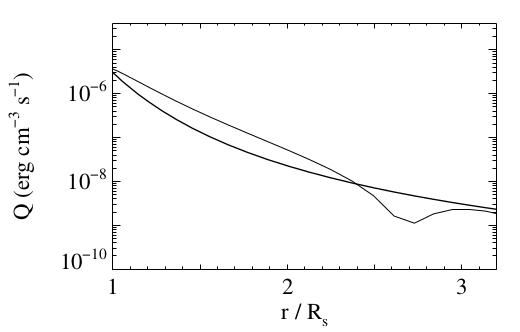
\includegraphics[width=0.65\textwidth]{figuras/heating_dmitruk_2002.png}
\end{center}
\caption{Función de calentamiento por unidad de volumen en la baja corona obtenido con el modelo RMHD (línea gruesa) y con el modelo fenomenológico (línea delgada).}
\label{heating}
\end{figure}





%\section{Tasa de Disipación de Ondas de Alfvén}\label{tasa_final}


Reemplazaremos el término no lineal $\nabla \cdot (\boldsymbol{z}_\mp w_\pm)$ de la Ecuación \ref{bardo2} por el término fenomenológico de \citet{dmitruk_2002}, es decir $\nabla \cdot (\boldsymbol{z}_\mp w_\pm) \sim (2/L)\sqrt{w_\mp/\rho}w_\pm$. De esta forma estamos considerando que la tasa de disipación de densidad de energía ($w_\pm$) es controlada por la amplitud de la onda propagante en sentido opuesto $|\boldsymbol{z_\mp}| = 2 \sqrt{w_\mp/\rho}$ y por una longitud de correlación (L) entre las ondas. De esta forma introducimos a la derecha de la Ec. \ref{alfven_1} el término disipativo,
 
\begin{equation}
  \frac{\partial w_\pm}{\partial t} + \nabla \cdot [(\boldsymbol{v}\pm \boldsymbol{V}_A)w_\pm] = - \frac{w_\pm}{2}(\nabla \cdot \boldsymbol{v}) - \Gamma_{\pm} w_\pm \label{alfven_2}
\end{equation}
donde el último término corresponde a la disipación, donde la tasa queda determinada por
\begin{equation}
  \Gamma_{\pm} = \frac{2}{L}\sqrt{\frac{w_{\mp}}{\rho}}.
\end{equation}
Para que haya ondas contrapropagantes en las líneas magnéticamente abiertas, debemos introducir el término de reflexión de onda (R) debido a gradientes de densidad,

\begin{equation}
  \frac{\partial w_\pm}{\partial t} + \nabla \cdot [(\boldsymbol{v}\pm \boldsymbol{V}_A)w_\pm] = - \frac{w_\pm}{2}(\nabla \cdot \boldsymbol{v}) - \Gamma_{\pm} w_\pm \mp R\sqrt{w_- w_+}.\label{alfven_3}
\end{equation}
Si bien esta ecuación sigue dentro del enfoque WKB, posee ahora términos mas precisos.

Los términos de disipación de ondas de Alfvén serán los que generen inyección de energía a iones y electrones ($Q_i$ y $Q_e$). Si no consideramos otros términos de inyección entonces $Q_i + Q_e = \Gamma_+ w_+ + \Gamma_- w_-$ que equivale a la disipación total y por lo tanto a la ganancia total de energía de iones y electrones (esta ganancia se refiere a términos de ganancia no conservativas en las ecuaciones de conservación de energía de cada especie), que podemos expresar como:
\begin{equation}
  Q_i = f_p(\Gamma_+ w_+ + \Gamma_- w_-) \,\,\,\,\,\,\,\,\,\,\,\,\, Q_e = (1-f_p)(\Gamma_+ w_+ + \Gamma_- w_-),
\end{equation}
donde se entiende que $Q_i + Q_e$ es la disipación total, y $f_p$ corresponde a la fracción de energía de onda de Alfvén disipada en iones. El particionamiento de la disipación es un tema abierto, algunos enfoques pueden encontrarse en \citet{hollweg_1986} y \citet{vander_2014}, donde el particionamiento toma valores $f_p \sim 0.7$. 

Las ondas de Alfvén ejercen presión isotrópica \citep{jacques_1977}, la relación entre la presión de onda y la densidad de energía de onda es $P_A = (w_+ + w_-)/2$. Esta presión cumple el rol de acelerar el viento solar y debe ser considerada en la ecuación de momento (Ec. \ref{pre1}) junto con los otros términos de presión isótropa.


\section{Modelado MHD con calentamiento por disipación de ondas de Alfvén}

Esfuerzos recientes apuntan a desarrollar y testear modelos MHD 3D que incluyan a las ondas de Alfvén como el agente impulsor principal tanto para calentar el plasma como para acelerar el viento solar \citep{gombosi_2018}. En este contexto se desarrolló el modelo Alfvén Wave Solar Model (AWSoM;  \citet{vander_2014}). Este modelo MHD 3D de la corona solar es parte del Space Weather Modeling Framework (SWMF; \citet{swmf_2005}), y toma como único dato el campo magnético mediante magnetogramas, es decir la medición fotosférica de la componente radial del campo magnético. El modelo resuelve las ecuaciones MHD ideal (Ecs. \ref{conserv_densidad}-\ref{mhd_B}) junto con disipación de ondas de Alfvén (Ec. \ref{alfven_3}) y modela tanto la corona como la heliósfera interna.


Tal como fue introducido en la Sección \ref{turbulencia} y \ref{tasa}, este modelo aborda calentamiento de la corona solar al incluir la interacción no lineal de las ondas de Alfvén desde la cromosfera hacia el exterior y contrapropagadas (reflejadas) en las líneas magnéticamente cerradas lo que da como resultado una cascada turbulenta. Dentro de los agujeros coronales, no hay líneas de campo magnético cerradas, por lo tanto, no hay ondas de propagación opuesta. En cambio, un reflejo de las ondas que se propagan hacia el exterior (dada por gradientes de densidad) genera localmente ondas que se propagan hacia el Sol. Estas ondas contrapropagantes conducen a una tasa de disipación de turbulencia en los agujeros coronales generando calentamiento y acelerando el viento solar rápido.

Esta energía turbulenta disipada se distribuye entre protones y electrones utilizando teorías de amortiguación de onda lineal y calentamiento estocástico. El modelo incluye enfriamiento radiativo y la conducción de calor de electrones tanto colisional como no colisiona y no utiliza funciones de calentamiento ad-hoc.

A modo de ejemplo utilizaremos a continuación la rotación de Carrington CR2223 que se encuentra en un mínimo de actividad. A modo de ejemplificación de algunos de los resultados que provee el modelo 3D, seleccionamos mapas de latitud en función de longitud (llamados mapas de Carrington) para una altura especifica. 

Se ejemplifica en la Figura \ref{resultados1} mapas de Carrington de la temperatura electrónica $T_e$ (arriba), de la componente radial de la velocidad del viento solar $V_r$ (medio) y de la densidad electrónica (abajo), a la altura de $6 R_{\odot}$. En la primera se observan temperaturas mayores en las regiones polares. El mapa de velocidad del viento muestra un mínimo en la zona de la HCS, lo que conforma el viento solar lento. A medida que nos desplazamos desde latitudes ecuatoriales hacia los polos, la velocidad aumenta hasta alcanzar su máximo en la zona polar, conformando el viento solar rápido. Si bien a esta altura aún no se alcanzó la velocidad terminal ya se observa la relación 2:1 entre el viento rápido y el lento. El mapa de densidad electrónica $N_e$ a la misma altura muestra densidades máximas en la HCS y mínimas en la zona polar. Esto es consistentes con un viento solar lento y denso asociado al Streamer ecuatorial y un viento solar rápido y más tenue en la zona polar asociado a los agujeros coronales (en concordancia con datos de Ulyses, Fiug. \ref{ulysses}).

La Figura \ref{resultados2} muestra un mapa de Carrington la presión de onda Alfvén a bajas alturas. La zona mas oscura que denota relativamente baja presión se da dentro de la zona magnéticamente cerrada, y en rojo se muestra la zonas abiertas donde la presión es relativamente mas alta. Este mapa deja en evidencia que la disipación de ondas de Alfvén acelera el viento rápido, proveniente de la zona polar.


\begin{figure}%[ht]
\begin{center}
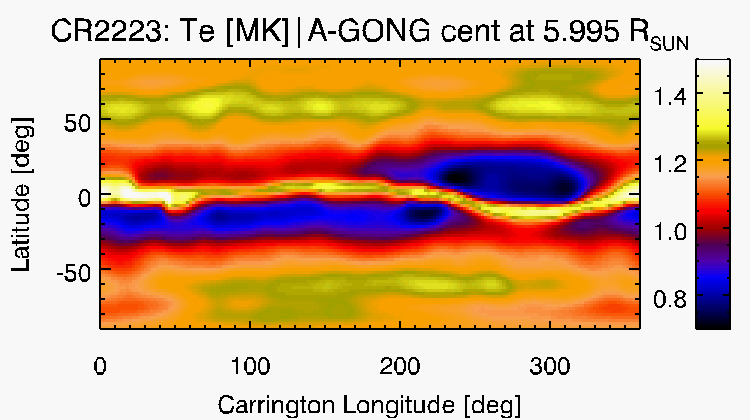
\includegraphics[width=0.6\textwidth]{figuras/map_Te_awsom_2223_cocent_extended_5_995_Rsun.png}
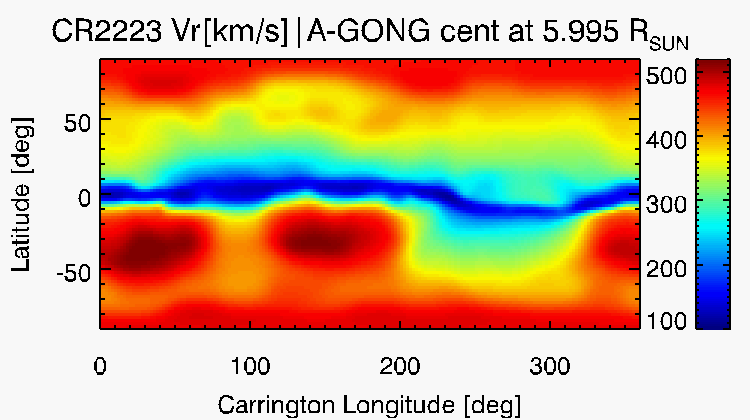
\includegraphics[width=0.6\textwidth]{figuras/map_Vr_awsom_2223_cocent_extended_5_995_Rsun.png}
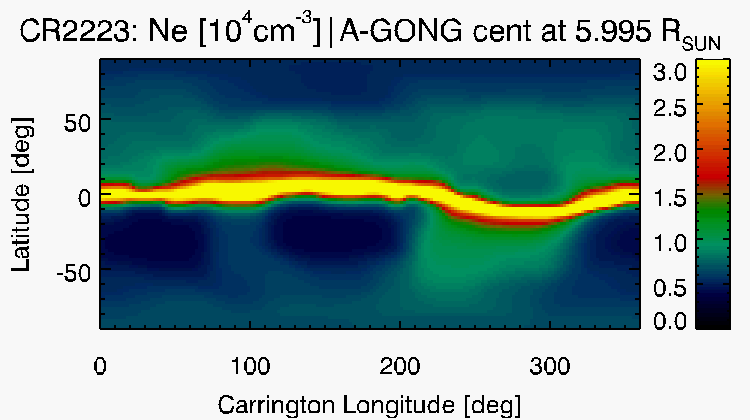
\includegraphics[width=0.6\textwidth]{figuras/map_Ne_awsom_2223_cocent_extended_5_995_Rsun.png}
\end{center}
\caption{Resultados del modelo AWSoM para CR2223 a $6 R_{\odot}$. Arriba se muestra un mapa de Carrington de la temperatura electrónica, en el medio un mapa de Carrington de la componente radial de la velocidad del viento solar y abajo un mapa de Carrington de la densidad electrónica.}
\label{resultados1}
\end{figure}


\begin{figure}%[ht]
\begin{center}
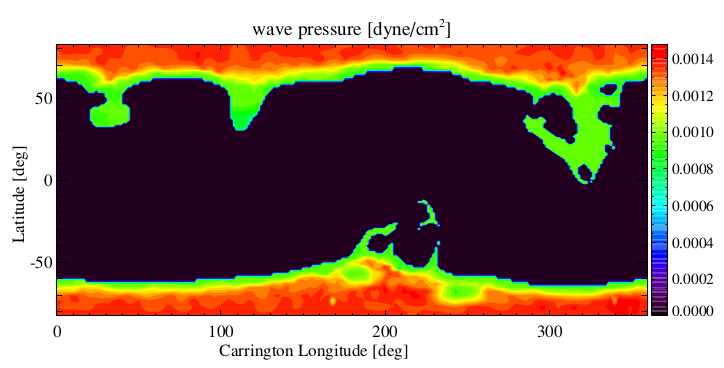
\includegraphics[width=0.5\textwidth]{figuras/presion_alfven_vander2010.png}
\end{center}
\caption{Mapa de Carrington de la presión de onda de Alfvén a $1.03 R_{\odot}$}
\label{resultados2}
\end{figure}



De esta forma queda evidenciado el hecho de que una cascada de energía turbulenta hacia escalas de pequeña longitud puede sostenerse gracias a ondas Alfvén reflejadas por la densidad media y los gradientes del campo magnético. Este mecanismo deposita energía de manera eficiente en la corona inferior. Esto proporciona un mecanismo de calentamiento robusto que puede explicar las altas temperaturas coronales observadas, explica la aceleración del viento en las zonas abiertas y explica la distribución significativa del calentamiento (por unidad de volumen) por debajo de $2R_\odot$ necesarios en los modelos del origen del viento solar.




\begin{comment}
\chapter*{Apéndice}
\begin{eqnarray}
  \nabla \cdot (\boldsymbol{a}\boldsymbol{b}) &=& \boldsymbol{a} \cdot \nabla \boldsymbol{b} + \boldsymbol{b}\nabla \cdot \boldsymbol{a} \label{apen_1}\\ 
  \boldsymbol{a} \times (\nabla \times \boldsymbol{b}) &=& (\nabla \boldsymbol{b})\cdot \boldsymbol{a}- \nabla \cdot (\boldsymbol{a}\boldsymbol{b})-\boldsymbol{b}\nabla \cdot \boldsymbol{a}  \label{apen_2}\\
  \nabla \times(\boldsymbol{a} \times \boldsymbol{b}) &=& \nabla \cdot (\boldsymbol{b}\boldsymbol{a}-\boldsymbol{a}\boldsymbol{b}) \label{apen_3}\\
  \nabla (\boldsymbol{a}\cdot \boldsymbol{b}) &=& (\nabla\boldsymbol{a})\cdot \boldsymbol{b}+(\nabla\boldsymbol{b})\cdot \boldsymbol{a} \label{apen_4}\\
  \nabla \cdot (\boldsymbol{a} \times \boldsymbol{b}) &=& \boldsymbol{b} \cdot \nabla \times \boldsymbol{a} - \boldsymbol{a} \cdot \nabla \times \boldsymbol{b} \label{apen_5} \\
  \boldsymbol{a}\times (\boldsymbol{b} \times \boldsymbol{c}) &=& \boldsymbol{a} \cdot \boldsymbol{c}\boldsymbol{b} - \boldsymbol{a}\cdot \boldsymbol{b}\boldsymbol{c} \label{apen_6}
\end{eqnarray}
\end{comment}





\bibliographystyle{spr-mp-sola}
\bibliography{bibliografia}

\end{document}







